\subsection{Drawer}\label{sec:launcher:drawer}
The drawer is a separate view that is situated in the left-hand side of the \textit{Home} activity.
Its main purpose is to allow \launcher users to apply a new colour-scheme to the installed \giraf applications.

The concept of the drawer is a component that can be shown and hidden at will.
This means that only part of the drawer is visible at all time; it can be dragged towards the centre of the screen to reveal its contents.
Apart from enabling the users to switch colours of their installed \giraf applications, it also contains various informative widgets.
These widgets includes a calendar for showing current day and date, a server connection indicator updating the synchronization status of the remote database\footnote{This connection indicator widget has no effect, since database synchronization is not implemented.}, and a logout button.\vagner{hmm... refer to the discussion about widgets not working?}
The implementations of these widgets are a part of \textit{Giraf Components}, a separate project in the \giraf system that handles customized Graphical User Interface components.
It should be utilized throughout all \giraf applications to make them look and feel the same.

Illustrations of the drawer in closed and opened positions can be seen in \cref{fig:drawerclosed,fig:draweropened} respectively.

\begin{figure}[h] % Billeder af draweren i åben og lukket tilstand
\centering
	\begin{subfigure}[b]{.48\textwidth}
	\centering
	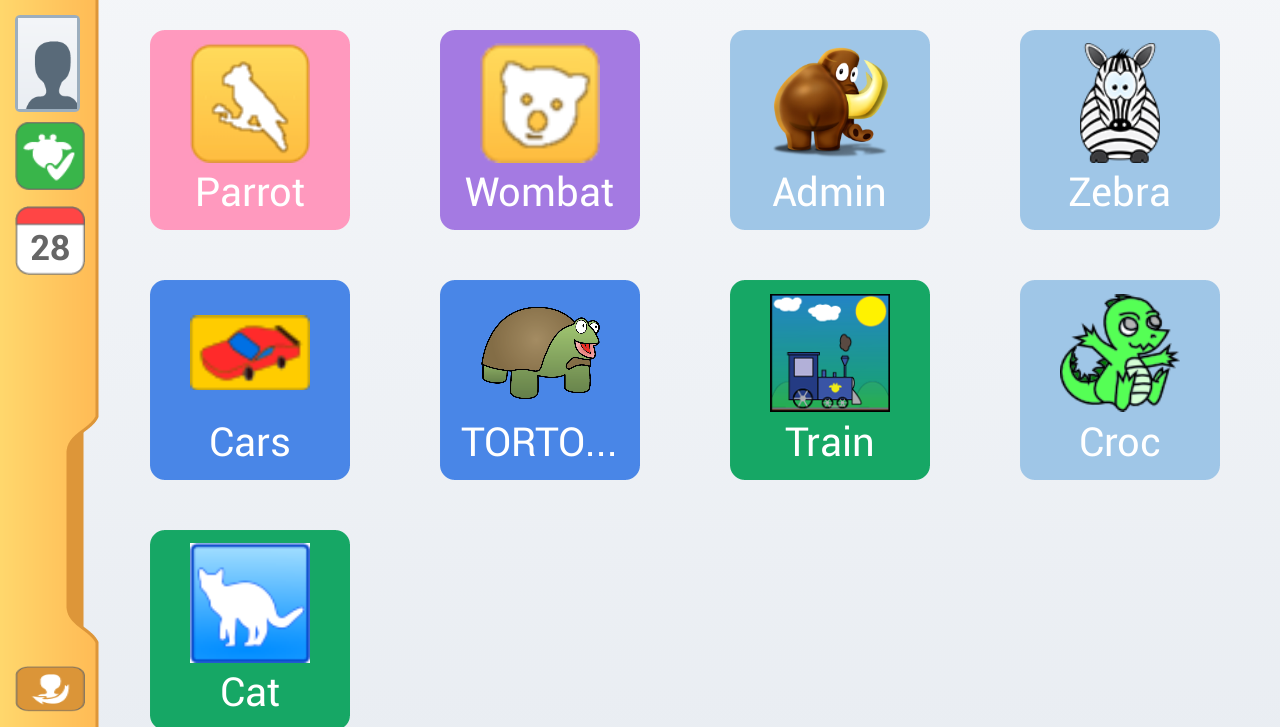
\includegraphics[width=\textwidth]{screenshots-old-giraf/giraf-homeactivity.png}
	\caption{Drawer closed.}
	\label{fig:drawerclosed}
	\end{subfigure}
	\hfill
	\begin{subfigure}[b]{.48\textwidth}
	\centering
	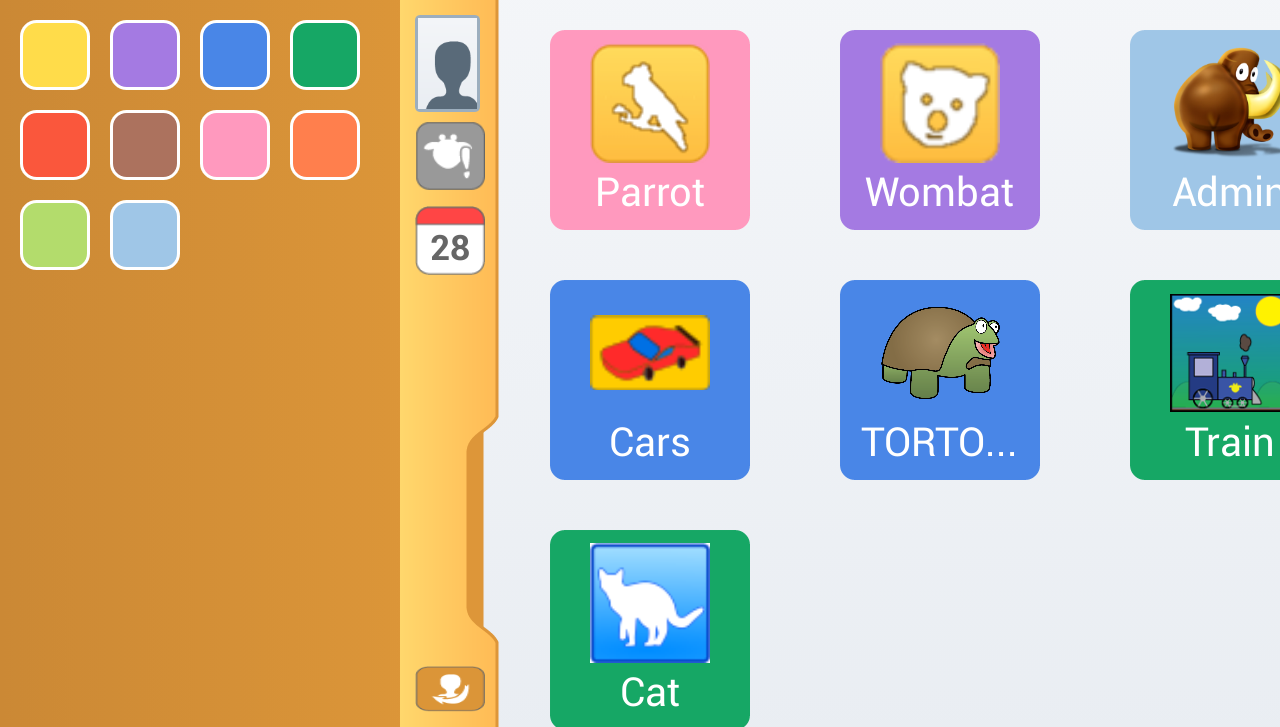
\includegraphics[width=\textwidth]{screenshots-old-giraf/giraf-drawer-fullyextended.png}
	\caption{Drawer fully extended.}
	\label{fig:draweropened}
	\end{subfigure}
\caption{States of the drawer component shown on \textit{Home} activity.}
\label{fig:drawerstates}
\end{figure}

As indicated by \cref{fig:drawerstates}, the drawer already meet the requirement that a colour can be dragged onto an application.
In spite of this, many deficiencies have been located, which are further enlightened by the following sections.

\subsubsection{Behaviour of the Drawer}\label{sec:drawer:behaviour}
The drawer opens by pressing and holding the handle (indentation) of the vertical bar (see \cref{fig:drawerclosed}) while sliding it to the right.
While being opened, the drawer pushes the application icons along with it to the right, resulting in some icons disappearing off-screen to the right.
Furthermore, the drawer stops sliding when pressure is released from the touch-screen, meaning it can be left in a half-open, half-closed state.
To change the colour of an application, a colour can be drag-and-dropped onto an application icon. 
The result is immediately apparent, as the colour framing the icon changes to the selected colour.

\subsubsection{Desired Improvements}
\thilemann{Skal vi skrive om andre forbedringer af de forskellige activities vi skriver om herover?}
Since no formal requirements are available and the project group have not yet held a meeting with the customers, the suggested improvements below is based on what we find to be natural requirements of such a User Interface component. 

\begin{itemize}
\item The drawer should be either open or closed. A half-open or half-closed state should result in the drawer popping into the state closest to its current position.
\item The drawer should close while a colour is being dragged, and open again when dropped.
\item The drawer should not push the application icons out of the screen.
\item The source code responsible for the animation of the drawer and the layout of the home activity should be re-factored in order to:
\begin{itemize}
\item take advantage of standard Android animations and layout features,
\item allow the activity to dynamically adjust according to display-size and
\item reduce the amount of clutter in the source code and improve readability.
\end{itemize}
\end{itemize}

The implementation of the improvements is described in \cref{sec:developments:drawerimprovements}.